\documentclass{beamer}
\beamertemplatenavigationsymbolsempty
\usepackage{amsmath, amssymb, hyperref, graphics}
\usepackage{tikz}
%\usepackage{mathpazo}
\usetikzlibrary{graphs}
\usetikzlibrary{graphs.standard}


\newcommand{\Z}{\mathbb{Z}}
\newcommand{\Q}{\mathbb{Q}}
\newcommand{\R}{\mathbb{R}}


\title{Graph Theory Lecture 3}




\begin{document}
\begin{frame}{Lecture 3}
  \begin{block}{Current plan: include algorithms}
    \begin{itemize}
    \item Next week: Eulerian and Hamiltonian Graphs
    \item 4 Lectures each of the last 3 units
    \end{itemize}
  \end{block}
  
    \begin{block}{Today: three quick hits}
\begin{itemize}
    \item Basic definitions
    \item Trees
    \item Applications to Chemistry
      \end{itemize}
    \end{block}
  
  \end{frame}

\begin{frame}[plain,c]

\begin{center}

\Huge

\usebeamercolor[fg]{frametitle}
Basic Definitions
\end{center}

\end{frame}




\begin{frame}{Basic graphs and concepts}
  \begin{itemize}
  \item The \emph{empty graph} $E_n$ has $n$ vertices and no edges
  \item The \emph{complete graph} $K_n$ has $n$ vertices, and each vertex is connected to every other.
  \item The \emph{path graph} $P_n$ has $n$ vertices $\{1,\dots,n\}$ with an edge between $i$ and $i+1$
    \item The \emph{cycle graph} $C_n$ has $n$ vertices $\{1,\dots, n\}$ with an edge between $i$ and $i+1$ and between $n$ and $1$.
  \end{itemize}

  \begin{block}{The Petersen Graph}
\begin{center}
    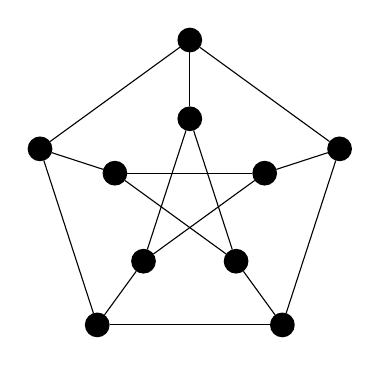
\begin{tikzpicture}[every node/.style={circle, draw, fill=black, inner sep=0pt, minimum width=4pt, thick}]
      \graph[clockwise, radius=2cm] {subgraph C_n [n=5,name=A]};
  \graph[clockwise, radius=1cm] {subgraph I_n [n=5,name=B]};

  \foreach \i in {1,2,3,4,5}{\draw (A \i) -- (B \i);}
  \newcounter{j}
  \foreach \i in {1,2,3,4,5}{%
  \pgfmathsetcounter{j}{ifthenelse(mod(\i+2,5),mod(\i+2,5),5)}
  \draw (B \i) -- (B \thej);
  }
 
\end{tikzpicture}
\end{center}
\end{block}
\end{frame}

\begin{frame}{Connected means we can ``get from any vertex to another''}
  \begin{definition}[Walk] Let $G$ be a simple graph.  A \emph{walk} in $G$ is a sequence of vertices $v_1, v_2, \dots, v_n$ so that $v_i$ is adjacent to $v_{i+1}$.  We we say the walk goes from $v_1$ to $v_n$.
    \end{definition}

  \begin{definition}[Connected] A graph $G$ is \emph{connected} if there is a walk between any two vertices $v$ and $w$ in $G$.
  \end{definition}

  \begin{block}{Definitions I won't use without explaining:}
    \begin{itemize}
    \item A \emph{trail} is a walk that doesn't repeat any edges
    \item A \emph{path} is a walk that doesn't repeat any vertices
    \end{itemize}
    \end{block}

\end{frame}
  
\begin{frame}{Bipartite graphs}
  \begin{definition}[Bipartite graphs] A graph $G$ is \emph{bipartite} if we can colour every vertex either blue or red so that every edge goes between a blue vertex and a red vertex.
  \end{definition}
  \begin{definition}[Complete bipartite graphs] The \emph{complete bipartite graph} $K_{m,n}$ consists of $m+n$ vertices, $m$ coloured red, $n$ coloured blue, and an edge between any red vertex and and any blue vertex.
  \end{definition}

  \begin{block}{Examples}
    \end{block}
\end{frame}

\begin{frame}{Another way to characterise bipartite graphs}  
  \begin{lemma}A graph $G$ is bipartite if and only if it doesn't have any cycles of odd length (i.e., subgraphs of the form $C_{2k+1}$).
    
    \end{lemma}
  \begin{block}{Bipartite $\implies$ no odd cycles:}
    Subgraphs of bipartite graphs are bipartite
  \end{block}
  \begin{block}{No odd cycles $\implies$ Bipartite:}
Try to colour $G$ by distance from $v$   
\end{block}
  \begin{definition}[Distance]Let $G$ be connected, and let $v,w$ be two vertices.  The \emph{distance from $v$ to $w$} is the least number of edges in any walk from $v$ to $w$.
    \end{definition}


  
\end{frame}

\begin{frame}[plain,c]

\begin{center}

\Huge

\usebeamercolor[fg]{frametitle}
Trees
\end{center}

\end{frame}

\begin{frame}{A forest is a bunch of trees}
  \begin{figure}
            \includegraphics[width=\textwidth]{Pictures/forest.png}
\caption{A forest of three trees}
  \end{figure}

  \begin{definition}\begin{itemize}
    \item A \emph{forest} is a graph without cycles
    \item A \emph{tree} is a connected graph without cycles
    \end{itemize}
  \end{definition}
\end{frame}

\begin{frame}{The Treachery of Definitions (After Magritte)}
  \begin{figure}
    \includegraphics[width=.85\textwidth]{Pictures/NotATree.jpg}
    \caption{Ceci n'est pas un arbre  (This is not a tree)} 
\end{figure}
\end{frame}

\begin{frame}{$\lfloor 13/2\rfloor$ ways of looking a tree (After Wallace Stevens)}
  \begin{block}{Proposition:} Let $G$ be a graph with $n$ vertices.  The following are equivalent.
    \begin{enumerate}
    \item $G$ is a tree (i.e., $G$ connected but has no cycles)
    \item There is a unique path in $G$ between any two vertices
    \item $G$ is connected and has $n-1$ edges
    \item $G$ has no cycles and has $n-1$ edges
    \item $G$ is connected, but removing any edge disconnects $G$
    \item $G$ has no cycles, but adding any edge creates a cycle
      \end{enumerate}
  \end{block}
  \begin{block}{Informally: Trees are Goldilocks graphs}
    \begin{itemize}
\item    Trees have enough edges: they're connected \\
\item    Trees don't have too many edges: they have no cycles
  \end{itemize}
\end{block}

\end{frame}

\begin{frame}{Make like a tree and get out of here (After Biff Tannen)}

  \begin{definition}[Tree]Let $T$ be a tree.  A vertex $v\in T$ is a \emph{leaf} if it has degree 1.\end{definition}
\begin{lemma}Let $T$ be a tree with $2\leq n<\infty$ vertices.  Then $T$ has at least two leaves. \end{lemma}

\begin{block}{Proof 1: See title of slide.}
Pick an edge, and try to ``leave'' -- that is, walk as far as you can.
  \begin{itemize}
  \item No loops, so you'll never return to where you are
  \item Finitely many vertices, so it can't go on forever
  \end{itemize}
Eventually you'll get stuck -- that's a leaf.
\end{block}
\end{frame}
\begin{frame}{Pruning Trees}
  \begin{block}{Part of Proposition:} If $T$ is a tree with $n$ vertices, then $T$ has $n-1$ edges.
  \end{block}
  \begin{block}{Proof: Induct on $n$}
    \begin{itemize} \item Base case: $n=1$
      \item Now assume that all trees with $n-1$ vertices have $n-2$ edges
      \item If $T$ is a tree with $n$ vertices, it has a leaf $v$ (by Lemma)
        \item Delete $v$ and the edge next to it to get a new tree $T^\prime$ 
        \item $T^\prime$ has $n-1$ vertices, so $n-2$ edges, so $T$ has $n-1$ edges.
          \end{itemize}
    \end{block}
\end{frame}

\begin{frame}{Another use of the handshaking lemma}
  \begin{block}{Part of Proposition:}
    If $G$ is a connected graph with $n$ vertices and $n-1$ edges, then $G$ is a tree.
  \end{block}
  \begin{block}{Proof: induct on $n$}
    \begin{itemize}
    \item Base case: $n=1$
    \item Assume proposition is true for all graphs with $n-1$ vertices
    \item Since $G$ is connected, it has no vertices of degree 0
    \item Use handshaking to show $G$ must have a vertex $v$ of degree 1
    \item Delete $v$ and the edge next to it to get a new graph $G^\prime$
    \item $G^\prime$ is a tree, so $G$ must have been as well
    \end{itemize}
  \end{block}
  \end{frame}

\begin{frame}[plain,c]

\begin{center}

\Huge

\usebeamercolor[fg]{frametitle}
Chemistry
\end{center}

\end{frame}


\begin{frame}{Chemical formulas encode degree sequences}
\includegraphics[width=\textwidth]{Pictures/periodictablebig.jpg}
\begin{center} $\begin{array}{c|cccc}
  \text{Atom} & C & N & O & H \\ \hline 
  \text{Degree} & 4 & 3 & 2 & 1
  \end{array}$ \end{center}
\end{frame}


\begin{frame}{Shortcuts around Carbon and Hydrogen}
  \begin{figure}
    \includegraphics[width=.5\textwidth]{Pictures/Caffeine3d.png}
    \includegraphics[width=.5\textwidth]{Pictures/Caffeine_structure.png}
    \caption{Two pictures of Caffeine}
  \end{figure}
  \begin{itemize}
  \item Unlabelled vertices are Carbon
  \item Hydrogen not drawn; inferred to make degrees correct
  \end{itemize}
\end{frame}

\begin{frame}{Isomers are graphs with the same degree sequence}
  \begin{definition}An \emph{Alkane} is a molecule with formula $C_nH_{2n+2}$
  \end{definition}
  \includegraphics[width=.8\textwidth]{Pictures/Hydrocarbons.jpg}
\begin{definition}[Isomer] Two different molecules are \emph{isomers} if they have the same chemical formula.
 \end{definition}
  
\begin{block}{Lemma: Any alkane is a tree.}
  Proof: Handshaking.
  \end{block}
\begin{block}{Question: How many isomers does $C_5H_{12}$ have?}
\end{block}
\end{frame}

\end{document}
